\documentclass[11pt, a4paper]{report}

\usepackage[utf8]{inputenc}
\usepackage[margin=0.5in]{geometry}
\usepackage{fancyvrb}
\usepackage{amsmath}
\usepackage{amsfonts}
\usepackage{amssymb}
\usepackage{enumitem}
\usepackage{listings}
\usepackage{natbib}
\usepackage{amsmath, amsthm, amssymb}
\usepackage{ upgreek }
\usepackage{ tipa }
\usepackage{graphicx}

\begin{document}
\title{Practica02: PSeint}
\author{
  Introducci\'on a la Programaci\'on\\
  \texttt{10/Noviembre/2018}
  \and
  G\'omez Guti\'errez Uzziel\\
  \texttt{17-011-0019}
}
\date{}
\maketitle

\section*{Ejercicio 1}

\begin{figure}[!ht]
\begin{center}
  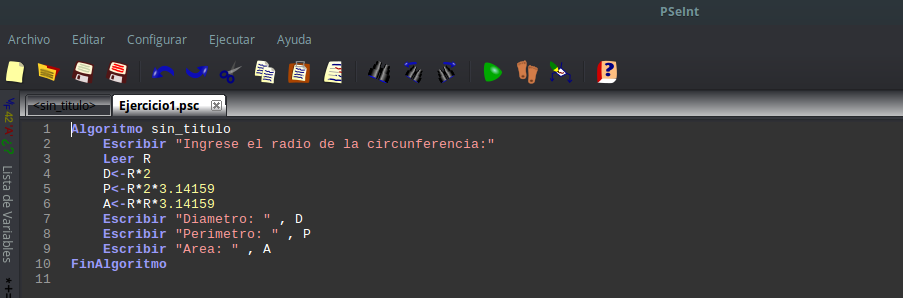
\includegraphics[width=0.9\textwidth]{ejercicio1.png}
  \caption{Pseudoc\'odigo ejercicio 1}
\end{center}
\end{figure}

\begin{figure}[!ht]
\begin{center}
  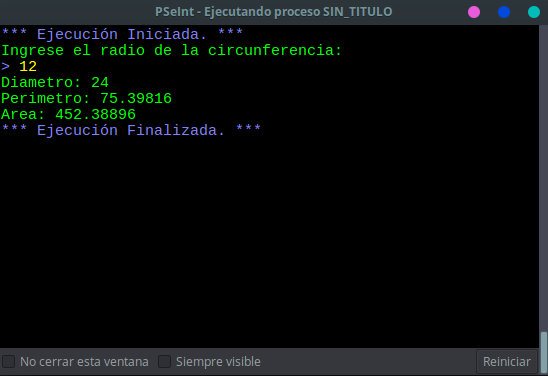
\includegraphics[width=0.6\textwidth]{respuesta1.png}
  \caption{Respuesta ejercicio 1}
\end{center}
\end{figure}
 	
 \newpage	
\section*{Ejercicio 2}

\begin{figure}[!ht]
\begin{center}
  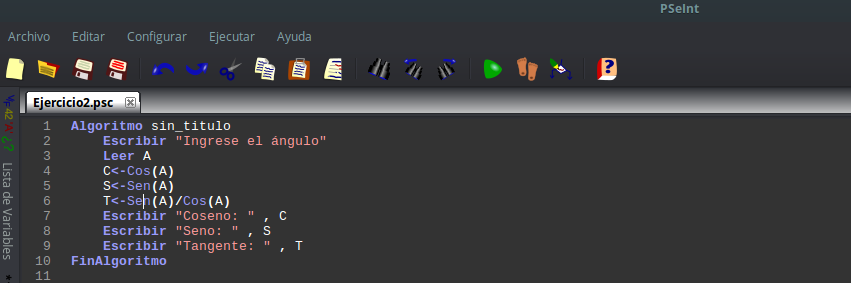
\includegraphics[width=0.9\textwidth]{ejercicio2.png}
  \caption{Pseudoc\'odigo ejercicio 2}
\end{center}
\end{figure}

\begin{figure}[!ht]
\begin{center}
  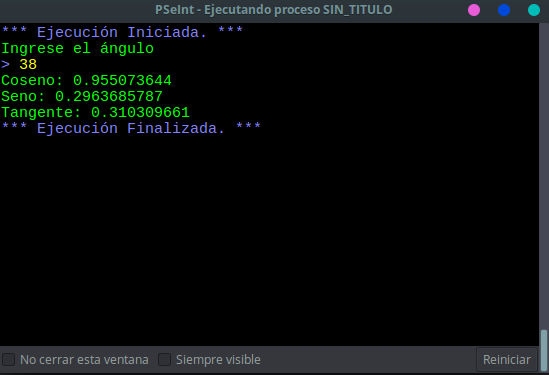
\includegraphics[width=0.6\textwidth]{respuesta3.png}
  \caption{Respuesta ejercicio 2}
\end{center}
\end{figure}

\newpage
\section*{Ejercicio 3}

\begin{figure}[!ht]
\begin{center}
  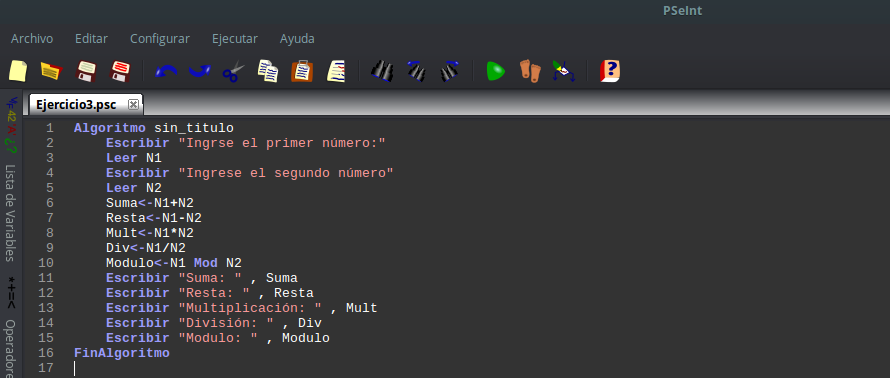
\includegraphics[width=0.9\textwidth]{ejercicio3.png}
  \caption{Pseudoc\'odigo ejercicio 3}
\end{center}
\end{figure}

\begin{figure}[!ht]
\begin{center}
  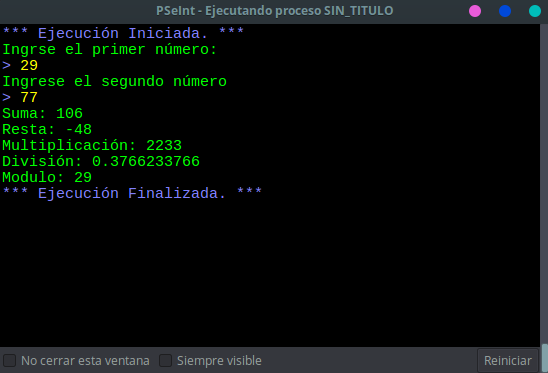
\includegraphics[width=0.6\textwidth]{respuesta4.png}
  \caption{Respuesta ejercicio 3}
\end{center}
\end{figure} 

\newpage
\section*{Ejercicio 4}

\begin{figure}[!ht]
\begin{center}
  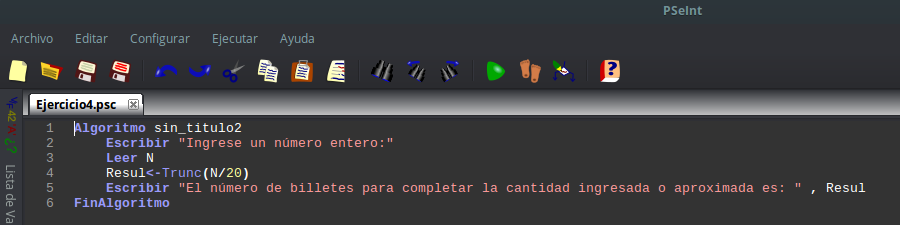
\includegraphics[width=0.9\textwidth]{ejercicio4.png}
  \caption{Pseudoc\'odigo ejercicio 4}
\end{center}
\end{figure}

\begin{figure}[!ht]
\begin{center}
  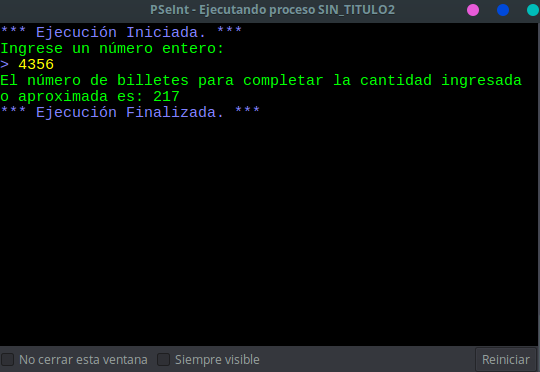
\includegraphics[width=0.6\textwidth]{respuesta5.png}
  \caption{Respuesta ejercicio 4}
\end{center}
\end{figure}

\newpage
\section*{Ejercicio 5}

\begin{figure}[!ht]
\begin{center}
  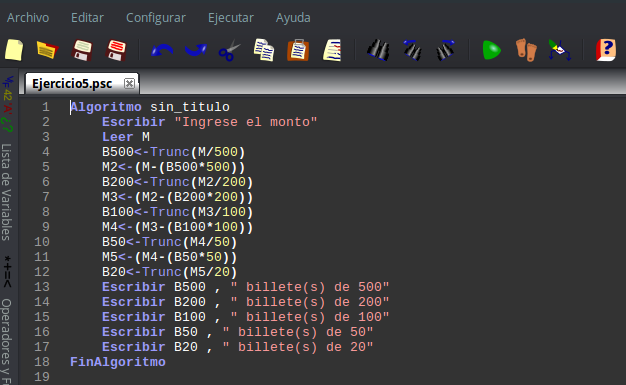
\includegraphics[width=0.9\textwidth]{ejercicio5.png}
  \caption{Pseudoc\'odigo ejercicio 5}
\end{center}
\end{figure}

\begin{figure}[!ht]
\begin{center}
  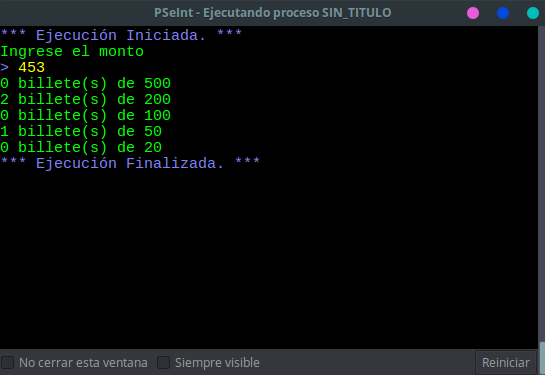
\includegraphics[width=0.6\textwidth]{respuesta6.png}
  \caption{Respuesta ejercicio 5}
\end{center}
\end{figure}

\end{document}